% Copyright (c) 2021 Eclipse Arrowhead Project
%
% This program and the accompanying materials are made available under the
% terms of the Eclipse Public License 2.0 which is available at
% http://www.eclipse.org/legal/epl-2.0.
%
% SPDX-License-Identifier: EPL-2.0

With the major themes of the \GlossaryHyperRef{framework-arrowhead}{Arrowhead framework} now established, we proceed to outline its most significant concepts in detail.
Each subsection of this section \GlossaryHyperRef{description}{describes} one of these concepts, which are as follows:

\vfill

\noindent\begin{tabularx}{\textwidth}{@{} p{0.9cm} p{4.3cm} X @{}}

\ref{sec:concepts:stakeholder} & \textbf{\nameref{sec:concepts:stakeholder}} & A person or \GlossaryHyperRef{organization}{organization} engaged in an \GlossaryHyperRef{entity}{entity} or undertaking. \\
\ref{sec:concepts:entity}      & \textbf{\nameref{sec:concepts:entity}}      & An \GlossaryHyperRef{artifact}{artifact} that can be distinguished from all other artifacts. \\
\ref{sec:concepts:device}      & \textbf{\nameref{sec:concepts:device}}      & A physical \GlossaryHyperRef{entity}{entity} with the \GlossaryHyperRef{capability}{capability} of hosting \GlossaryHyperRef{system}{systems}. \\
\ref{sec:concepts:system}      & \textbf{\nameref{sec:concepts:system}}      & A \GlossaryHyperRef{instance-software}{software instance} able to exercise the \GlossaryHyperRef{capability}{capabilities} of its hosting \GlossaryHyperRef{device}{device}. \\
\ref{sec:concepts:service}     & \textbf{\nameref{sec:concepts:service}}     & A set of \GlossaryHyperRef{operation}{operations} \GlossaryHyperRef{provider-service}{provided} by a \GlossaryHyperRef{system}{system} for other systems to \GlossaryHyperRef{consumer-service}{consume}. \\
\ref{sec:concepts:sos}         & \textbf{\nameref{sec:concepts:sos}}         & A set of \GlossaryHyperRef{system}{systems} that jointly facilitate new \GlossaryHyperRef{capability-system}{capabilities}. \\
\ref{sec:concepts:local-cloud} & \textbf{\nameref{sec:concepts:local-cloud}} & A \GlossaryHyperRef{cloud}{cloud} with a \GlossaryHyperRef{boundary-local}{local boundary} and \GlossaryHyperRef{resource-local}{local resources}.\\
\ref{sec:concepts:solc}        & \textbf{\nameref{sec:concepts:solc}}        & A set of \GlossaryHyperRef{cloud-local}{local clouds} that jointly facilitate new \GlossaryHyperRef{capability-system}{capabilities}.\\
\ref{sec:concepts:network}     & \textbf{\nameref{sec:concepts:network}}     & A set of \GlossaryHyperRef{device}{devices} whose \GlossaryHyperRef{system}{systems} can \GlossaryHyperRef{communication}{communicate}.\\
\ref{sec:concepts:interface}   & \textbf{\nameref{sec:concepts:interface}}   & A \GlossaryHyperRef{boundary}{boundary} that can be crossed by the \GlossaryHyperRef{message}{messages} of certain \GlossaryHyperRef{protocol}{protocols}.\\
\ref{sec:concepts:policy}      & \textbf{\nameref{sec:concepts:policy}}      & A set of \GlossaryHyperRef{constraint}{constraints} that must be satisfied for an activity to be permitted.\\
\ref{sec:concepts:protocol}    & \textbf{\nameref{sec:concepts:protocol}}    & A \GlossaryHyperRef{description}{description} of how \GlossaryHyperRef{message}{messages} may be sent between \GlossaryHyperRef{entity}{entities}.\\

\end{tabularx}

\subsection{Stakeholder}
\label{sec:concepts:stakeholder}

A \GlossaryHyperRef{stakeholder}{stakeholder} is a person or \GlossaryHyperRef{organization}{organization} with \GlossaryHyperRef{stake}{stake} in an \GlossaryHyperRef{entity}{entity} or undertaking with relevance to the \GlossaryHyperRef{framework-arrowhead}{Arrowhead framework}.
In this context, we understand \textit{stake} to refer to any type of engagement or commitment.
The concept is illustrated in Figure \ref{fig:stakeholder}, which also lists five reasons why a given person or organization could be considered to be a stakeholder.
We refer to these reasons as \GlossaryHyperRef{role-stakeholder}{\textit{roles}}.

\vfill

\begin{figure}[ht!]
  \centering
  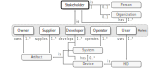
\includegraphics[scale=0.9]{figures/stakeholder}
  \caption{
    The stakeholder as either a person or organization, where each such stakeholder takes on one ore more distinct roles.
    The depicted roles is not an exhaustive list.
    \GlossaryHyperRef{hid}{HID} is an abbreviation for \GlossaryHyperRef{device-human-interface}{Human Interface Device}.
  }
  \label{fig:stakeholder}
\end{figure}

The roles occupied by a given stakeholder dictates what \GlossaryHyperRef{entity}{entities} that person or organization will interact with, as well as the nature of those interaction.
In Figure \ref{fig:stakeholder}, (1) \GlossaryHyperRef{owner}{owner}, (2) \GlossaryHyperRef{supplier}{supplier}, (3) \GlossaryHyperRef{developer}{developer}, (4) \GlossaryHyperRef{operator}{operator} and (5) \GlossaryHyperRef{user}{user} are named explicitly, but more roles are likely to be relevant, such as (6) \GlossaryHyperRef{acquirer}{acquirer} and (7) \GlossaryHyperRef{maintainer}{maintainer}, (8) \GlossaryHyperRef{builder}{builder}, (9) \GlossaryHyperRef{researcher}{researcher} and (10) \GlossaryHyperRef{architect}{architect}.
The listed ten names should be used rather than any synonyms when referring to these particular roles.
Please refer to the \hyperref[sec:glossary]{glossary} for their definitions.
If this document is read electronically, each role name can be clicked to be taken to its definition.

\subsection{Entity}
\label{sec:concepts:entity}

An \GlossaryHyperRef{entity}{entity} is an \GlossaryHyperRef{artifact}{artifact} that can be distinguished from all other artifacts.
We use the word \textit{artifact} to refer to any object or thing, physical or intangible.
As depicted in Figure \ref{fig:entity}, this means that an entity always has an \GlossaryHyperRef{identity}{identity}.

\vfill

\begin{figure}[ht!]
  \centering
  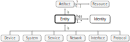
\includegraphics[scale=0.9]{figures/entity}
  \caption{
    The entity as an artifact with an identity.
    An entity or artifact may or may not be considered to be a \GlossaryHyperRef{resource}{resource}, in which case it is deemed to be of value to a \GlossaryHyperRef{stakeholder}{stakeholder}.
    The group of entity types is not exhaustive.
    Other examples are \GlossaryHyperRef{cloud-local}{local clouds}, certain \GlossaryHyperRef{data}{data}, \GlossaryHyperRef{policy}{policies} and \GlossaryHyperRef{profile}{profiles}.
  }
  \label{fig:entity}
\end{figure}


Note that having an identity is not the same as being associated with an \GlossaryHyperRef{identifier}{identifier}, which is a name, number or other value referring to an entity.
It is enough that any such identifier is possible to produce for an artifact to count as an entity.
That being said, certain \GlossaryHyperRef{identification}{identification} requirements, perhaps related to security, performance or discoverability, may make it practically unfeasible not to use identifiers.

\subsection{Device}
\label{sec:concepts:device}

A \GlossaryHyperRef{device}{device} is a physical \GlossaryHyperRef{entity}{entity} with the significant \GlossaryHyperRef{capability}{capability} of being able to host at least one \GlossaryHyperRef{system}{system}, each of which may be given the opportunity to exercise the capabilities of that device.
Examples of capabilities include moving robotic arms, reading from sensors, running \GlossaryHyperRef{procedure-software}{software procedures}, and sending \GlossaryHyperRef{message}{messages}. 
Every device consists of \GlossaryHyperRef{component-hardware}{hardware components}.
While there are no limits to what components can make up a device, each device must always have (1) \GlossaryHyperRef{unit-memory}{memory}, (2) \GlossaryHyperRef{unit-compute}{compute} and (3) \GlossaryHyperRef{interface-device}{interfacing} components, as shown in Figure \ref{fig:device}.

\vfill

\begin{figure}[ht!]
  \centering
  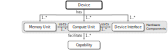
\includegraphics[scale=0.9]{figures/device}
  \caption{
    The device as an entity with hardware components, together facilitating one or more capabilities.
    Devices must be able to host systems, even if not made explicit by this figure.
    Other examples of hardware components part of a device could be sensors, actuators, compute accelerators, or batteries.
  }
  \label{fig:device}
\end{figure}

A device \GlossaryHyperRef{hosting-system}{\textit{hosts}} a system by executing the \GlossaryHyperRef{software}{software} of that system in one or more of its compute units.
Devices must be able to host systems, or they must be considered as hardware components.
While it may seem unintuitive to consider certain machines as components, such as large pumping complexes or vehicles with only manual controls, the \GlossaryHyperRef{framework-arrowhead}{Arrowhead framework} is meant to facilitate automation through the use of interconnected devices with compute capabilities.
If a machine cannot run software, making it able to host systems, that capability must be added before it can play a meaningful role in an Arrowhead context.
Consequently, machines without system hosting capabilities must either be considered as components or not be considered from the perspective of Arrowhead at all.

\subsection{System}
\label{sec:concepts:system}

A \GlossaryHyperRef{system}{system} is an \GlossaryHyperRef{identification}{identifiable} \GlossaryHyperRef{instance-software}{software instance} that is able to exercise the \GlossaryHyperRef{capability}{capabilities} of its \GlossaryHyperRef{hosting-system}{hosting} \GlossaryHyperRef{device}{device}.
As shown in Figure \ref{fig:system}, systems consists of \GlossaryHyperRef{component-software}{software components}.
Some significant such components are (1) \GlossaryHyperRef{state-software}{states}, (2) \GlossaryHyperRef{procedure-software}{procedures} and (3) \GlossaryHyperRef{interface-system}{system interfaces}.
A system with these components should be able to \GlossaryHyperRef{consumer-service}{consume} and/or \GlossaryHyperRef{provider-service}{provide} \GlossaryHyperRef{service}{services}, or it must be referred to as an \GlossaryHyperRef{system-isolated}{\textit{isolated system}}.

\begin{figure}[ht!]
  \centering
  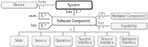
\includegraphics[scale=0.9]{figures/system}
  \caption{
    The system as a collection of related software components, able to facilitate new capabilities.
    While not made explicit by this figure, all software components are \GlossaryHyperRef{hosting-software}{hosted} by either hardware or software components, which means that they use and/or are maintained by those components.
    Examples of software components could be operating systems, file systems, software libraries, programming language runtimes, databases or virtual machines.
  }
  \label{fig:system}
\end{figure}

This rather open-ended definition of ``system'' makes it possible for such to be realized in many ways.
A system may or may not run in its own operating system process, use a certain virtual machine, and so on.

\subsection{Service}
\label{sec:concepts:service}

A \GlossaryHyperRef{service}{service} is an \GlossaryHyperRef{identification}{identifiable} set of \GlossaryHyperRef{operation-service}{operations} \GlossaryHyperRef{provider-service}{provided} by a \GlossaryHyperRef{system}{system}.
Other systems may consume such a service by sending a \GlossaryHyperRef{message}{message} to, or \GlossaryHyperRef{invocation-operation}{\textit{invoking}}, an operation part of that service.
If the sent message is valid, the providing system may use its \GlossaryHyperRef{capability}{capabilities} to satisfy the request of the sending system.
As depicted in Figure \ref{fig:service}, operations receive messages via \GlossaryHyperRef{interface-provider}{provider interfaces} and send their own messages via \GlossaryHyperRef{interface-consumer}{consumer interfaces}.

\vfill

\begin{figure}[ht!]
  \centering
  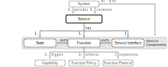
\includegraphics[scale=0.9]{figures/service}
  \caption{
    The service as a set of operations made available via a provider interface, making it possible for a providing system to offer use of its capabilities to consuming systems.
    Every entity depicted in this figure, except for the \textit{System} and the \textit{Capability}, may be a \GlossaryHyperRef{component-software}{\textit{Software Component}}.
  }
  \label{fig:service}
\end{figure}

When a provider interface receives a message, as described in Section \ref{sec:concepts:interface}, it must \GlossaryHyperRef{routing-message}{route} it to the operation it targets.
The operation must then ensure that the message adheres to its \GlossaryHyperRef{protocol-operation}{protocol} and satisfies all of its \GlossaryHyperRef{policy-operation}{policies}, after which it must handle the request described by the message.
As described further in Sections \ref{sec:concepts:policy} and \ref{sec:concepts:protocol}, the policies ensure that the message is handled under desirable conditions, while the protocol ensures that it can be interpreted by the operation.
For example, a policy could demand that a valid authorization token is included in the message, while a protocol could depend on the message \GlossaryHyperRef{encode}{encoding} a certain \GlossaryHyperRef{type-data}{data type}.

\subsection{System-of-Systems}
\label{sec:concepts:sos}

A \GlossaryHyperRef{system-of-systems}{system-of-systems} is an \GlossaryHyperRef{identification}{identifiable} set of at least two \GlossaryHyperRef{system}{systems}, together facilitating one or more \GlossaryHyperRef{capability-system}{capabilities} none of the constituent systems could have on its own.
The facilitation of new capabilities is accomplished by the systems providing services and/or consuming each other's services.

While it may seem as if consuming services would hardly be enough for new capabilities to always emerge, it actually is the case.
For example, let us assume that a system has the capability of turning on and off a light.
That system also provides a service allowing for other systems to request that the light be turned on or off.
If a different system can successfully consume that service, it also gains the capability of turning on and off that particular light.
As a new system now may control that particular light, a new capability has emerged.

\subsection{Local Cloud}
\label{sec:concepts:local-cloud}

A \GlossaryHyperRef{cloud-local}{local cloud} is a \GlossaryHyperRef{system-of-systems}{system-of-systems} able to execute given tasks through the use of a pool of \GlossaryHyperRef{resource}{resources}.
The resource pool of a local cloud could contain 3D-printers, autonomous unmanned vehicles, conventional servers, or anything else producing a value on demand.
As depicted in Figure \ref{fig:local-cloud}, the local cloud is distinct from other types of \GlossaryHyperRef{cloud}{clouds} by having at least one \GlossaryHyperRef{boundary-local}{local boundary} and one \GlossaryHyperRef{resource-local}{local resource}, which means that it is physically tied to a concrete location.
A local cloud could be engaged in manufacturing, repairs, heating, electricity distribution, workspace monitoring, drone fleet control, among many other possible kinds of physical activities.
A local cloud may be stationary or mobile.
A cloud that has no resources or boundaries tied to any particular physical locations should be referred to as a \GlossaryHyperRef{cloud-virtual}{\textit{virtual cloud}}.

\vfill

\begin{figure}[ht!]
  \centering
  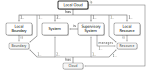
\includegraphics[scale=0.9]{figures/local-cloud}
  \caption{
    The local cloud as a regular cloud with at least one local boundary and one local resource.
  }
  \label{fig:local-cloud}
\end{figure}

That a local cloud has a boundary means that a distinction is being made between \GlossaryHyperRef{system}{systems} inside and outside the cloud.
A boundary being local means that the distinction is being made by a physical \GlossaryHyperRef{attribute}{attribute}, such as device location, type of device, or physical attachment to a certain \GlossaryHyperRef{entity}{entity}.
Boundaries may be protected, which means that measures are in place to guarantee security, safety, real-time characteristics, or other local cloud attributes.
The resources of a local cloud may be of any type, from virtual compute resources to physical drills or pumps.
A system managing a resource may be referred to as a \GlossaryHyperRef{system-supervisory}{\textit{supervisory system}}.

\subsection{System-of-Local-Clouds}
\label{sec:concepts:solc}

A \GlossaryHyperRef{system-of-local-clouds}{system-of-local-clouds} is two or more \GlossaryHyperRef{cloud-local}{local clouds} that \GlossaryHyperRef{consumer-service}{consume} each other's \GlossaryHyperRef{service}{services} to facilitate new \GlossaryHyperRef{capability-system}{capabilities}.
It is similar to the local cloud, with the exception of its \GlossaryHyperRef{subsystem}{subsystems} are \GlossaryHyperRef{cloud-local}{local clouds} instead of plain \GlossaryHyperRef{system}{systems}.
A system-of-local-clouds may have its own \GlossaryHyperRef{boundary-cloud}{boundaries} in addition to those of its constituent local clouds.
Those boundaries are formed by attributes shared by all the constituent local clouds, such as certificates issued by the same organization, or physical attachment to the same network bus.
A system-of-local-clouds cannot have resources beyond those of its constituent clouds, however.

\subsection{Network}
\label{sec:concepts:network}

A \GlossaryHyperRef{network}{network} is an \GlossaryHyperRef{identification}{identifiable} set of two or more \GlossaryHyperRef{device-end}{end devices}, \GlossaryHyperRef{connection}{connected} such that any \GlossaryHyperRef{system}{systems} they host are able to \GlossaryHyperRef{communication}{communicate}.
As shown in Figure \ref{fig:network}, end devices may be \GlossaryHyperRef{interconnection}{interconnected} via \GlossaryHyperRef{device-intermediary}{intermediary devices}.

\vfill

\begin{figure}[ht!]
  \centering
  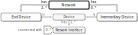
\includegraphics[scale=0.9]{figures/network}
  \caption{
    The network as a set of connected end devices, potentially interconnected by intermediary devices.
  }
  \label{fig:network}
\end{figure}

Both end devices and intermediary devices are regular \GlossaryHyperRef{device}{devices}, which means that they have \GlossaryHyperRef{interface-device}{device interfaces} through which they can send and receive \GlossaryHyperRef{message}{messages}.
Only \GlossaryHyperRef{device-connected}{\textit{connected} devices} can pass messages between their interfaces, however.
Intermediary devices pass on messages toward their intended end devices instead of handling them themselves.
Examples of intermediary devices are routers, switches, and firewalls.
Device interfaces used exclusively for passing on messages are referred to as \GlossaryHyperRef{interface-network}{network interfaces}.
The term ``end device'' should only be used when a distinction needs to be made between end and intermediary devices.

\subsection{Interface}
\label{sec:concepts:interface}

An \GlossaryHyperRef{interface}{interface} is an \GlossaryHyperRef{identification}{identifiable} \GlossaryHyperRef{boundary}{boundary} where \GlossaryHyperRef{message}{messages} of certain \GlossaryHyperRef{protocol}{protocols} can pass between a \GlossaryHyperRef{connection}{connection} and an \GlossaryHyperRef{entity}{entity}, between entities, or between an entity and a person.
As outlined in Figure \ref{fig:interface}, there are three types of interfaces of particular relevance, (1) \GlossaryHyperRef{interface-device}{device interfaces}, (2) \GlossaryHyperRef{interface-system}{system interfaces}, and (3) \GlossaryHyperRef{interface-service}{service interfaces}.

\vfill

\begin{figure}[ht!]
  \centering
  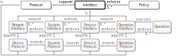
\includegraphics[scale=0.9]{figures/interface}
  \caption{
    The interface as a boundary only messages of a certain protocol may cross.
    Service, system and device interfaces enable services, systems and devices to communicate with entities beyond their own boundaries.
  }
  \label{fig:interface}
\end{figure}

These three types of interfaces form three levels.
At each level, if a received message satisfies its protocol, it is routed towards its designated recipient.
If the message does not satisfy its protocol, it is ignored, replied to with an error message, or some other action is performed.
As depicted in Figure \ref{fig:service}, provider interfaces route messages to \GlossaryHyperRef{operation-service}{service operations}, which may handle them by sending new messages via consumer interfaces.

Each of these interface levels depend on the layer below it, with the exception of the device interface at the bottom.
As each interface supports its own set of protocols, each interface layer must support a protocol that extends that of the below layer.
A device interface may, for example, support the IP \cite{deering2017internet} protocol via Ethernet \cite{iso202188023}, a system interface the HTTP \cite{fielding2014hypertext} protocol via TCP \cite{postel1981transmission}, and a service interface a custom HTTP extension allowing for a target service operation to be specified.
Note that the protocol at each layer may consist of multiple protocols extending each other, as in this example.
A particular chain of protocols supported by a device, system or service is referred to as a \GlossaryHyperRef{stack-protocol}{\textit{protocol stack}}.
The protocol stack of the system in the previous example would be Ethernet, IP, TCP and HTTP, from the bottom and up.

%\newpage

\subsection{Policy}
\label{sec:concepts:policy}

A \GlossaryHyperRef{policy}{policy} is an \GlossaryHyperRef{identification}{identifiable} set of \GlossaryHyperRef{constraint}{constraints} that must be satisfied for a certain activity to be permitted.
Policies may be concerned with authorization, contracts, economic goals, and so on.
As depicted in Figure \ref{fig:policy}, the type of policy of highest relevance to the \GlossaryHyperRef{framework-arrowhead}{Arrowhead framework} is the one enforced by \GlossaryHyperRef{operation-service}{service operations}.

\begin{figure}[ht!]
  \centering
  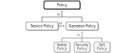
\includegraphics[scale=0.9]{figures/policy}
  \caption{
    The policy as a set of constraints.
    The types of constraints depicted are to be considered as examples of possible constraints.
    \GlossaryHyperRef{qos}{QoS} is an abbreviation for \GlossaryHyperRef{service-quality-of}{quality of service}.
  }
  \label{fig:policy}
\end{figure}

An operation policy must be satisfied for a system to be allowed to \GlossaryHyperRef{consumer-service}{consume} a particular \GlossaryHyperRef{operation-service}{service operation}.
Failing to satisfy a policy should mean that the consumer in question is notified about the specific policy or policies being violated.
Policies may be associated with any \GlossaryHyperRef{entity}{entities} that receive \GlossaryHyperRef{message}{messages}, such as \GlossaryHyperRef{interface}{interfaces}.

\subsection{Protocol}
\label{sec:concepts:protocol}

A \GlossaryHyperRef{protocol}{protocol} is an \GlossaryHyperRef{identification}{identifiable} \GlossaryHyperRef{description}{description} of how certain \GlossaryHyperRef{message}{messages} may be sent between \GlossaryHyperRef{entity}{entities} as dictated by zero or more \GlossaryHyperRef{state-protocol}{states}.
Received messages may be rejected for violating a current state, or cause a state to be updated.
States may also be updated by events not related to messages. 
As shown in Figure \ref{fig:protocol}, a protocol may be defined as an \GlossaryHyperRef{protocol-extensible}{extension} of another protocol, as well as be constrained by certain \GlossaryHyperRef{profile-protocol}{profiles} and \GlossaryHyperRef{encoding}{encodings}.

\begin{figure}[ht!]
  \centering
  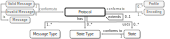
\includegraphics[scale=0.9]{figures/protocol}
  \caption{
    The protocol as set of state and message types, constrained by profiles and encodings.
  }
  \label{fig:protocol}
\end{figure}

A profile narrows down what a particular protocol is permitted to express, for example by requiring that authorization tokens be included in requests, or that a certain message payload semantics be observed.
Adding a profile to a protocol not already conforming to it produces a new protocol.
An encoding introduces a \GlossaryHyperRef{system-type}{type system} in which message payloads can be expressed.
If a protocol defines its messages without referring to an encoding, it is considered to have a \textit{custom} encoding.
